14. \begin{figure}[ht!]
\center{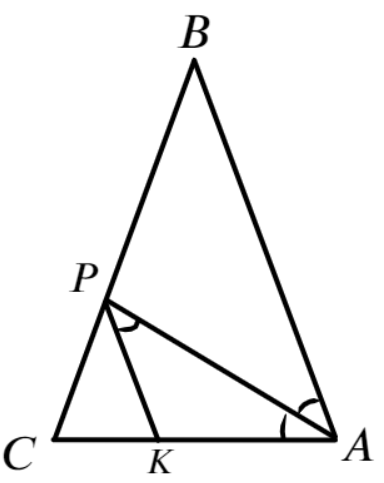
\includegraphics[scale=0.35]{g14.png}}
\end{figure}\\
Треугольник $ABC$ равнобедренный, поэтому $\angle A=\angle C =72^\circ.$ Так как $AP$ является биссектрисой, $\angle PAC=\angle PAB=72^\circ:2=36^\circ.$ Прямые $AB$ и $PK$ параллельны, $AP$ секущая, поэтому углы $KPA$ и $PAB$ равны как накрест лежащие, откуда $\angle KPA=36^\circ.$\\
